\documentclass[paper=a4, fontsize=11pt]{jhwhw} % A4 paper and 11pt font size
\usepackage{amsmath,amsfonts,amsthm, amssymb} % Math packages
\setlength\parindent{0pt} % Removes all indentation from paragraphs - comment this line for an assignment with lots of text
\usepackage{graphicx}
\usepackage{verbatim}
\usepackage{enumerate}
\usepackage{mathtools}
\usepackage{color}
\newcommand\SetSymbol[1][]{\:#1\vert\:}
\providecommand\given{} % to make it exist
\DeclarePairedDelimiterX\Set[1]\{\}{\renewcommand\given{\SetSymbol[\delimsize]}#1}
\usepackage{listings}

\definecolor{dkgreen}{rgb}{0,0.6,0}
\definecolor{gray}{rgb}{0.5,0.5,0.5}
\definecolor{mauve}{rgb}{0.58,0,0.82}

\lstset{frame=tb,
    language=Java,
    aboveskip=3mm,
    belowskip=3mm,
    showstringspaces=false,
    columns=flexible,
    basicstyle={\small\ttfamily},
    numbers=none,
    numberstyle=\tiny\color{gray},
    keywordstyle=\color{blue},
    commentstyle=\color{dkgreen},
    stringstyle=\color{mauve},
    breaklines=true,
    breakatwhitespace=true,
    tabsize=3
}



\begin{document}
\title{MP2}
\author{Ben Haines}

\section{Task 1: Feature Selection}
\subsection{Top 20 Words}
\subsubsection{Information Gain}
\begin{verbatim}
bland
nt
delici
mediocr
perfect
decent
rude
amaz
bad
overpr
disappoint
terribl
averag
favorit
worst
meh
hype
overr
love
horribl
\end{verbatim}
\subsubsection{Chi Square}
\begin{verbatim}
bland
mediocr
rude
decent
nt
bad
overpr
terribl
delici
worst
averag
disappoint
meh
overr
perfect
hype
amaz
horribl
lack
poor
\end{verbatim}

My final vocabulary contained 1780 unique unigrams. The resulting corpus after feature
selection contained 54286 reviews.

\subsection{Implementation}
In the code below, getPosDF returns the number of positive reviews the given token appears in.
\subsubsection{Information Gain}
\begin{lstlisting}[ basicstyle=\small]
public double InformationGain(Token tkn) {
    double term1 = 0.0;
    double term2 = 0.0;
    double term3 = 0.0;

    //Calc probabilities
    double y1_given_t = tkn.getPosDF()/tkn.getDF();
    double y0_given_t = 1 - y1_given_t;
    double y1_given_no_t = (numPos - tkn.getPosDF())/(m_reviews.size() - tkn.getDF());
    double y0_given_no_t = 1 - y1_given_no_t;
    double p_t = tkn.getDF()/m_reviews.size();
    double p_no_t = 1 - p_t;

    //Calculate term 1
    term1 += p_y0 * Math.log(p_y0);
    term1 += p_y1 * Math.log(p_y1);

    //Calculate term 2
    if (y0_given_t != 0) {
        term2 += y0_given_t * Math.log(y0_given_t);
    }
    if (y1_given_t != 0) {
        term2 += y1_given_t * Math.log(y1_given_t);
    }

    term2 *= p_t;

    //Calculate term3
    if (y0_given_no_t != 0) {
        term3 += y0_given_no_t * Math.log(y0_given_no_t);
    }
    if (y1_given_no_t != 0) {
        term3 += y1_given_no_t * Math.log(y1_given_no_t);
    }

    term3 *= p_no_t;

    return -term1 + term2 + term3;
}
\end{lstlisting}

\subsubsection{Chi-Square Score}
\begin{lstlisting}[ basicstyle=\small]
public double ChiSquareScore(Token tkn) {
    double A = tkn.getPosDF();
    double B = numPos - A;
    double C = tkn.getDF() - A;
    double D = (m_reviews.size() - numPos) - C;

    double numerator = (A + B + C + D) * Math.pow((A*D - B*C),2);
    double denominator = (A + C) * (B + D) * (A + B) * (C + D);

    return numerator / denominator;
}

\end{lstlisting}

\section{Task 2: Naive Bayes}
Lowest Ratio Words:
\begin{verbatim}
agr,-4.08896626809487
ine,-4.08896626809487
conver,-3.4423391031698163
sen,-3.4423391031698163
tasteless,-2.7821668395147627
unaccept,-2.749885644455242
aok,-2.717486992760117
overr,-2.4726931472074734
uninspir,-2.465259385859568
flavorless,-2.4478542987238665
insult,-2.315732708474327
stale,-2.2942385568537382
unimpress,-2.2769768439641087
mediocr,-2.1721336331580963
rude,-2.1186646659153947
bouncer,-2.056868352254339
worst,-2.0512134123690915
arrog,-2.0118860026007113
lacklust,-2.000358989574732
horribl,-2.0000557577140787
\end{verbatim}

Highest Ratio Words
\begin{verbatim}
flawless,3.476356115850656
radic,2.922411653682097
unpretenti,2.488536103757392
pur,2.3895433741137015
molecular,2.3895433741137015
gastronomi,2.3790830276887984
unforgett,2.2796634695711386
handsdown,2.2584229415611414
luscious,2.2407546374278287
mmmmm,2.0185805227373006
kimch,2.0000786073519787
scrumptious,1.994832005600136
thee,1.8896724764875756
achatz,1.88085265008446
marvel,1.8512898706661058
chee,1.8099343248768154
canada,1.7381750662282744
nom,1.6917065638310262
mmmm,1.6767511504916008
cali,1.6733151848577261
\end{verbatim}

The above rankings do make sense in terms of their ability to distinguish positive reviews from negative ones. Most of the words have very strong positive or negative connotations. Things like "flawless" would clearly suggest a positive review and "worst" a negative one. Without having done this analysis not all of the words are necessarily obvious though. I would not have predicted "mmmm" was one of the strongly distinguishing words but it makes sense in retrospect. The only words that don't make immediate sense to me are "canada", "cali", and "kimchee".

\subsection{Precision-Recall Curve}
In the following plot the color of the lines indicate the smoothing parameter $\delta$ used.
It is clear that different values for the smoothing parameter $\delta$ do produce different precision/recall tradeoffs. Increasing $\delta$ leads to a less discriminative classifier. As a result we tend to have lower precision for a given level of recall. This is reflected in the graph. It does take a fairly significant change in order to produce different results. The difference between values of 0.1 and 20 are very minimal.



\section{Task 3: k Nearest Neighbor}
\subsection{Implementation}
Generating Projection Vectors: I generate the vectors with python and write them to a csv which is then loaded when KNN is run. The vectors are only generated once.
\begin{lstlisting}
import numpy as np
import csv

f = open('projectionVectors.txt','w')
for i in range(5):
    x = np.random.uniform(-1.0, 1.0, 1780)
    for j in x:
        f.write(str(j)) 
        f.write(',') 
    f.write('\n') 
f.close() 
\end{lstlisting}

\begin{figure}[h]
    \center
    \caption{Precision Recall Curves}
    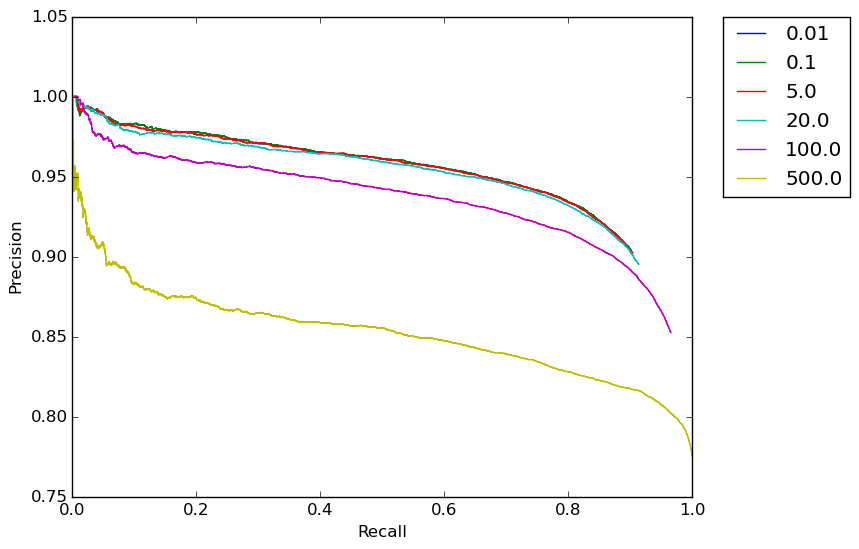
\includegraphics[scale=.7]{curves}
\end{figure}


Hashing Reviews: Before KNN begins all of the reviews in the search space are hashed using the projection vectors and added to a map keyed on this hash which stores the separate buckets. m\_projections contains the $\ell$ randomly generated vectors produced by the python code above. 
\begin{lstlisting}
public void HashReviews() {
    for (Post p : m_reviews) {
        ArrayList<Integer> hashVector = HashReview(p);

        if (m_buckets.containsKey(hashVector)) {
            m_buckets.get(hashVector).add(p);
        }
        else {
            HashSet<Post> val = new HashSet();
            val.add(p);
            m_buckets.put(hashVector, val);
        }
    }
}

public ArrayList<Integer> HashReview(Post p) {
    ArrayList<Integer> hashVector = new ArrayList<>();
    for (ArrayList<Double> projection : m_projections) {
        Double dotProd = p.innerProduct(projection);
        Integer bit = dotProd >= 0 ? 1 : 0;
        hashVector.add(bit);
    }

    return hashVector;
}
\end{lstlisting}

\subsection{Query Runtime and Results}
The time taken to execute the query for the five provided documents was 8.004412364 seconds for brute force KNN and 0.335724263 seconds for the random projection KNN. This is a very significant performance increase. We can see from the results below that in most cases the random projection heuristic seems to produce acceptable results. Most of the nearest results for a given query are similar both in tone and in the type of restaurant that they describe. Two of the queries return duplicate results. This happened because the program searched both the testing and training folders for neighbors and there was a duplicate file in these folders. Additionally, one of the query reviews was already in the teesting folder. This returned a result with a similarity score of 1. 
\begin{itemize}
\item Query 1
\begin{enumerate}
\item Score: 1.0\\
Result: Ahhh tapas, the small plates that contain individual tiny bites of joy. Cafe Ba-Ba-Reeba does their versions very well.In a group of 8, celebrating a birthday, many of the tapas were sampled and many drinks were to be had. Four of us split a pitcher of peach sangria, which was very good, each of us got two full glasses and there was a little top off to spare. As far as the food I personally took bites of:Bacon wrapped dates (5/5)Steak skewers (4/5)Spicy Potatotes (4/5)Fried Green Peppers (3/5) andPaella Valenciana (5/5)Braised short ribs w/mashed potatoes (5/5)Dessert - Chocolate Truffle Cake (3/5)You can't go wrong with bacon wrapped dates. The steak skewers and spicy potatoes were more impressive because of the sauce pairings. The fried green peppers were good, just not much to them, not a punch in the bite like I like my tapas. The paella was my favorite paella ever, mostly because paella usually comes with seafood and this one did not. Also it was done well. The braised short ribs I got to myself and every mouthful was very succulent and exactly like I would have wanted and was expecting. The chocolate cake was standard, nothing impressive, but good all the same. Service was around, clearing plates and making sure we got what all of our orders. Very impressive, especially since the concept of tapas induces a higher service standard than restaurants with the normal three plates.I can't wait to take the Mister here to show him how to eat like we do in España.
\item Score: 0.3722193249766118\\
Result: I absolutely loved our experience here. We made reservations earlier in the week for a Friday seating at 6 p.m. Good thing we did because the place was fairly packed and busy the entire time we were there.We came to celebrate my recent promotion and it was the perfect spot - very fun atmosphere and ambiance. It was just my boyfriend and I but this would be great for a group. We got seated right away and ordered the blackberry sangria. We each had about three glasses and I thought it was well worth the price. For the two of us we ordered the following off the menu:-patatas bravas: amazing and flavorful. Not too spicy but stills packs a punch.- goat cheese in marinara sauce: a personal favorite. I love the combination between the two and with some toasted bread you can't go wrong.-dates wrapped in bacon: everyone talks about these and they are not to be missed. The savory sweet aspect is awesome.-beef short rib with potatoes and brussels sprouts: short rib was fork tender and melt in your mouth-scallop dish: broth is great and very fragrant.With both of us checking into Yelp, we each got a dessert tapas for free. We tried the chocolate truffle cake and chocolate crema. Perfect sizes and the chocolate was fairly rich.The bill was around \$60, but we left full, satisfied, and in a sangria haze. Only recommendation would be to order 2 tapas at a time. Our 5 came out pretty fast and we were feeling a tiny bit overwhelmed with a table full of food!
\item Score: 0.36594068034082117\\
Result: Great tapas and nothing is bad that I have had from short ribs to seared tuna. The deserts are too small and the chocolate cake is just fudge so I would avoid the deserts. My favorite is figs wrapped in bacon because the bacon is always cooked well and the seet figs just melt in your mouth.
\item Score: 0.35832117304495525\\
Result: So full. Can't breathe.I love this place! It is always packed, but with the crowd comes a lively, energetic environment... *The traditional sangria is excellent, pitcher is a perfect size for 2-3 people* spicy potatoes, calamari, bacon wrapped dates, short rib with mashed potatoes, any of the meal and cheese samples, and who doesn't love more cheese... The hot goat cheese in red sauce is to die for as well. * the churros are no longer on the menu (sobbing), but they have an excellent flan and a butterscotch (??) dessert that is not to be missed. I would come here just to eat the spicy potatoes in that savory sauce and have a glass of sangria at the bar. The food is just consistently that good. ~40\$ per person or so, but no one will leave hungry or soberFun for groups and dates, not ideal for out of town parents who can't read the menu without a flashlight :-0
\item Score: 0.3296156718669713\\
Content: I'm a huge fan of the Tapas at Cafe Ba-Ba-Reeba. It is consistently good each time I stop by. The sangria is definitely a little weak, but the food makes up for it. I would recommend the bacon wrapped dates, the goat cheese tomato dip and of course the Paella! Great date restaurant, but I am not a big fan of Tapas in large groups. Give it a try.
\end{enumerate}
\item Query 2:
\begin{enumerate}
\item Score: 0.3113893102096704\\
Result: A few years ago, when I heard that Bill and Giuliana Rancic were opening up a LEYE Italian-themed restaurant, I'll admit, my eyes rolled a bit.  The star power of the couple definitely brought a buzz, and you add in the ability of the Melman family to turn a restaurant into a "see and be seen" place, but for some of their previous works (ala Hub 51 and Paris Club), the food seemed to take a backseat to the ambience and atmosphere.  So, I went into RPM the first time around pretty skeptical.  My first visit completely changed that - the food is well done, the pastas, fresh and handmade, offer a good choice of solidly cooked traditional options and dressed up more unique dishes.  I haven't tried some of the bigger secondi options yet, but mean to at some point in the future.  So about a month ago (hence the title "late thoughts", I checked out Wild Cub at the House of Blues.  Thankfully, seeing a show at the HOB leaves you with a plethora of nearby after-show eats, especially after an all-ages show.  So we headed over to RPM again, looking forward to some excellent fresh-made pasta.Fritto MistoWe started with the fritto misto, which ended up being the low point of the meal.  The shellfish aspects were fresh, but just a bit on the greasy side.  A bit disappointing, but thankfully the meal just got better after that.  Beef CarpaccioIt's not often that I'm in the mood for something like steak tartar or beef carpaccio, but for some reason it sounded enticing.  The beef was perfectly sliced, and the addition of the mushrooms added a nice textural contrast and a balance of flavor that was enhanced even more by the shaved pecorino cheese.  Scattered pieces of arugula gave a nice bite, and overall the extra ingredients didn't detract from the natural umami of the beef.  Lobster RavioliBucatiniSo two apps and two pastas was the perfect amount of food for the two of us.  I went with the lobster ravioli, cooked in a spinach-based green shell.  The ravioli was reasonably filled to get in a decent chunk of lobster, mostly claw meat,  The sauce, a light red sauce just adds enough flavor to the ravioli to complement the ravioli.  My fiancee's dish, "Mama DePandi's" Bucatini has become her go-to dish at RPM, and for good reason.  It's a simple dish - some fresh-made bucatini (a thick, tubular pasta with just the narrow hollow center) tossed with a freshly made pomodoro sauce.  The sweetness of the tomatoes really comes out in the sauce, and it's perfectly dressed.  Hints of basil and garlic round out the dish nicely.  So while you may be drawn towards some of the more unique sounding dishes on the menu (the squid ink pasta, the english pea risotto), the more traditional pastas have been the best here, IMO (I've also had the bolognese, and it was great!)Happiness comes in small packages, as long as there's hazelnut gelato inside, so save room for dessert.  And ask for the "chocolate ball".  The Tartufo is essentially a solid chocolate core, surrounded by gently flavored hazelnut gelato and held together by a crisp, nutty chocolate shell.  It is the perfect mix of flavors, textures, and temperatures in a dessert.  It's a good size for a number of people to share.  It is on my list of the best desserts (if not the best) dessert I've had in the city (that you can get consistently).   Surprisingly, RPM has turned into less of a scene restaurant than it's neighbors across the street, but still has a chic vibe.  But it's the food that stands out and is the highlight of this spot.  I give it a 4 stars, docked only bc it's just a tad on the pricier side, but if you order the right things, it's well worth it.Pics and more up at:eatinginchicago2014.word…
\item Score: 0.29540630986755934\\
Result: Went here with an old friend I hadn't seen in over five years, and our waiter Ryan was immediately attentive to the fact that we were here to catch up and enjoy a long friendly meal and conversation.  He paced the plates perfectly, and even expressed his concern that the pumpkin ravioli came too soon as we hadn't quite cleared the grape apple salad.  We didn't send a single plate back with a spot of food or sauce on it... and even licked the bowl of the pumpkin ravioli clean, it was like an f'n dessert mid-meal!!!  Back to the beginning, we started with the meatballs over polenta... the polenta was whipped super light and it's creaminess complimented the super meaty meatballs perfectly. From there things only got better.  We split the grape and apple salad and moved onto the pumpkin ravioli... (I am going back later this week just to have this dish once again!)  I cannot even begin to describe it, other than what I wrote above.  Finally we finished with the Steak and Eggs... The "sunny side up" or soft cooked egg was perfectly cooked inside the perfectly cooked, and I assume home-made ravioli wrapper... (or whatever you call that deliciously al-dente wheat based skin...)Come dessert, WTF, I cannot remember dessert... I remember it was really really good, but we were food comatose by this point and in sheer bliss... I checked out the menu online... We shared the warm gruyere donuts... again, f'n amazing!  Ryan our awesome waiter brought us an aperitif gratis and shared a few (more) laughs with us while we enjoyed the drinks before serving us with the check, which was beyond reasonable for such an amazing experience in life \& food!   Cheers L\&E we'll see you soon, if not sooner!
\item Score: 0.27493112701797323\\
Result: Had a really sweet and romantic meal outside here on my last night in Chicago this past Sunday. Ordered the margherita pizza which was really tasty and thin crust. No frills. Also had the veal meatballs and the ravioli. I loved both except the ravioli was a bit salty. My pomegranate martini was great and the babe ordered red wine which came with a funny regular cup just like in Italy. I think it's good for a breezy date night. Our server was a helpful and pretty girl whose name I didn't catch. Recommend.
\item Score: 0.27493112701797323\\
Result: Had a really sweet and romantic meal outside here on my last night in Chicago this past Sunday. Ordered the margherita pizza which was really tasty and thin crust. No frills. Also had the veal meatballs and the ravioli. I loved both except the ravioli was a bit salty. My pomegranate martini was great and the babe ordered red wine which came with a funny regular cup just like in Italy. I think it's good for a breezy date night. Our server was a helpful and pretty girl whose name I didn't catch. Recommend.
\item Score: 0.26852547031914353\\
Result: Amazing food, amazing service, great management. This place has never disappointed.
\end{enumerate}
\item Query 3:
\begin{enumerate}
\item Score: 0.22829051157893454\\
Result: I can't believe I haven't reviewed this place earlier! Fell in love with this place on my first visit and still love it. It started a few months ago...I walked in on a Friday night and my friend said that we'd have to wait. I was super hungry so I didn't mind and I'm glad I did instead of head to another restaurant on the block. The tacos are delicious. My favorite are the chicken tacos. They have a spicy kick and the meat is tender. The pork shoulder is my least favorite. Not sure if it's the pineapple I don't like or the meat. On to the plantains....I could eat these forever. They are perfectly grilled and the cheese, sauce, green onions...basically everything they put on top of the plantains make for a perfect combo. Also tried the pickled veggies on the side which I could have gone without. We also tried the bacon wrapped hot dog which was good but be warned...it's really messy! The drinks are delish as well and I love my tequila! If you go on a weekend night be prepared to wait. If you happen to find a spot at the bar then stay there! All the servers and bartenders are really friendly and provide great fast service so it doesn't really matter where you sit (just as long as you get a seat!). Last tip...CASH only.
\item Score: 0.22729609962346306\\
Result: I know that this place is supposed to be the greatest thing since sliced bread in Chicago; but you know what?  Its not!  Went here 1/16/2013 for a group/birthday party and really everything was just ehhh, and I have a couple of arrgghh you kidding me.  So I will start from the beginning, well pre-beginning because the idea of having a ticket system for a day, time and meal is just bull ****.  Here is why, say you want to go here; make reservation pay 500+ for tickets, now let say you get sick well to bad, that is the only time you can use ticket should have thought about that 3 months ago, oh yea you can try and sell it on CL or some other site but seriously good luck with that. No refunds you already payed for it so, I guess they really do not care is Grant really that hard up for money that he has to sucker customers by keeping tickets and changing reservation dates?  Any ways back to the evening The tree lined hallway was cool, nifty and a well executed idea; along with the super sweet hot chocolate when they took my coat.  I was seated along with the rest of the party, and offered the drink course with dinner which me and my date for evening declined and ordered a bottle of wine.  Most of the food that came out was okay at best the first course of the Sea Urchin, Toro and the Beef with Vegtable consomme was best dishes of the night.  Rest of dishes were okay not great and clearly forgettable a month or so later.  Now for the dish that has 50 different options to create your own was a great idea but if I ask you what all fifty options are; I expect you to answer me and not just say well it will be on the menu at the end.  Now this is about 3/4 of the way through the meal and I have been tasting my friends drinks that have been with the wine flight pairing and everything has been ungodly sweet, and I am not talking like a little sweet but sugar rush sweet.  So now its down to the grand finale and they do the chocolate explosion with cotton candy, caramel and cookies.  I take a couple bites and really this besides the little mess it made in some Jackson Pollack tribute of a look is just crap.  Hands down I have gotten super market chocolate that has been better.  Here is my advice, go some where else where the front of the house still takes reservations you do not have to buy stupid tickets that people low ball on CL, go to where it is not about name but a true adventure in finding excellent food.  I would say this place deserves the one Mitchlien star but that is it.
\item Score: 0.2041692024815178\\
Result: came here with my mother for lunch on a tuesday around 11:30am. we thought that since it was pretty early, there would probably be not be many people waiting to eat but when we got there it was VERY crowded and for a party of two, we waited for 40min. i feel like the wait is the only downside to this placeparking is very practical. the plaza where sushi gen is has its own parking lot and upon entering, u take a ticket and wait for a spot. since this little plaza consists of many restaurants, people are constantly leaving and arriving so its not difficult to land a parking spot. REMEMBER TO GET YOUR TICKET VALIDATED! (\$2 with validation, not bad at all)my mom ordered the lunch special chicken teriyaki \& sashimi combo (\$14) and i had the lunch special sashimi (\$15), both were YUUUMMMYY (: !! \$15 for the amount of sashimi i got was DEFFFFIIINITELY worth it AND it lived up to all the hype. and if u want more rice, they offer free refills which is a plus.
\item Score: 0.19433376067123756\\
Result: Avec is one of our favorites, except it can be impossible to get in and they don't take reservations (that's the main reason for 4 stars instead of 5).  We went last night early, at 5pm since we had tickets to a show and got in with no wait.  The food is amazing, there is nothing you can complain about with the food!!  We ordered the Dates, Foccia Bread, Pork Shoulder and the Hanger Steak for 3 people.  It was a lot of food!! We ended up taking some of it home, but we could have easily done with 1 plate less.Pros:- Food is amazing!!- Unique atmosphere- Reasonably pricedCons:- No reservations so you may end up waiting a while (alimentari just opened and they have a nice bar to wait at)- You sit at a table with other parties pretty crammed, so if you get stuck next to a bad crowd it could ruin your dinner
\item Score: 0.19433376067123756\\
Result: Avec is one of our favorites, except it can be impossible to get in and they don't take reservations (that's the main reason for 4 stars instead of 5).  We went last night early, at 5pm since we had tickets to a show and got in with no wait.  The food is amazing, there is nothing you can complain about with the food!!  We ordered the Dates, Foccia Bread, Pork Shoulder and the Hanger Steak for 3 people.  It was a lot of food!! We ended up taking some of it home, but we could have easily done with 1 plate less.Pros:- Food is amazing!!- Unique atmosphere- Reasonably pricedCons:- No reservations so you may end up waiting a while (alimentari just opened and they have a nice bar to wait at)- You sit at a table with other parties pretty crammed, so if you get stuck next to a bad crowd it could ruin your dinner
\end{enumerate}
\item Query 4:
\begin{enumerate}
\item Score: 0.2900410191269484\\
Result: I came here on a Sunday at 3:30 and there was still a long wait. That says alot about this brunch. I also love that they serve brunch this late. I ordered the Blu Jam Eggs Benedict and as Benny connoisuer, this definitely gets a stamp of approval! The hollandaise sauce was light and flavorful- not too salty. Instead of a thick cut piece of Canadian Ham, it was served with thinly sliced Black forrest ham AND crispy BACON.Oh and served with a side of country potates. Need I say more? This was all washed down with fresh squeezed OJ and freshly brewed coffee. My date got a breakfast burrito wrap that was also very tasty! I'm craving to come back here and try the french toast that I saw on the table next to me. Very cute place with excellent service and food!
\item Score: 0.25889498680355105\\
Result: Cochon, after one night of dining there, is now one of my all-time favorite restaurants.Since I worship at the temple of pork and pork-related foods, there really isn't a better concept for a restaurant than to have on centered around that very thing. So when I knew I was coming out to New Orleans, this restaurant became a top priority.I'm so glad I ate here.Our first meal, however, was not pork. It was fried alligator with chili-garlic aioli. I've had alligator before, and it wavers between delicious and rubber. This night's alligator was firmly in the middle. The sauce was spectacular, though, despite the overly chewy (even for gator) nature of the dish.The second dish was healthier, as I wanted something fresh to counteract the utter destruction of my body that was to follow. To my delight, the dish, cucumbers with herbs and vinegar, was simple, refreshing and sublime. Next came our first pork venture, barbecue ribs with watermelon pickles. What else can I say? Perfection. Great sauce, the rib meat was falling off the bone, and the pickles added a sweet and sour kick to the already tangy and sweet barbeque sauce. A winner.Next, deep fried boudin with fresh mustard and hot peppers. Boudin already rocks on its own, so to deep fry those suckers is to create one of the most delicious plates I've had in awhile. Pure awesomeness.The next dish was ham hocks with sweet potato, pickled greens and black eyed peas. The ham hocks came in their own jus, which made me happy. The flavors were really beyond description, a truly perfect blend of sweet, salty, and sour - all my favorite things, especially with pork.And then came the namesake dish of the restaurant - cochon with cracklins and turnips. Juicy and delicious, it truly knocked my socks off. And when cracklins (pork rinds) are just accompaniments for an already porky fabulous dish, you know you're in hog heaven.We finished with a root-beer parfait that was a nice, refreshing palate cleanser after the porky apocalypse that my stomach was subjected to.
\item Score: 0.23540974247176089\\
Result: Had dinner there but probably should have tried the one across the street and enjoyed a nice dinner.  It was just too packed to be enjoyable and feels like a wanna be place...We tried the grappa cured salmon w/ sweet \& sour cucumbers.  The salmon was ok, it was thick small pieces...but the sweet \& sour cucumbers were very good and refreshing.  For dinner, we had the Prosciutto d'Anitra pizza and the linguine w/ clam in white sauce.  The pizza was ok at best but the pasta was good, al dente.
\item Score: 0.23540974247176089\\
Result: Had dinner there but probably should have tried the one across the street and enjoyed a nice dinner.  It was just too packed to be enjoyable and feels like a wanna be place...We tried the grappa cured salmon w/ sweet \& sour cucumbers.  The salmon was ok, it was thick small pieces...but the sweet \& sour cucumbers were very good and refreshing.  For dinner, we had the Prosciutto d'Anitra pizza and the linguine w/ clam in white sauce.  The pizza was ok at best but the pasta was good, al dente.
\item Score: 0.23129729252566641\\
Result: one of the best sushi place ive been to!hamachi, tuna, aji, saba, uni, salmon, unagi! all so fresh and delicious! love sitting at the bar and just ordering piece by piece! unagi was warm, meaty and crispy! tuna melted in my mouth! everything was delicious!good friendly service too
\end{enumerate}
\item Query 5:
\begin{enumerate}
\item Score: 0.40094098450105714\\
Result: Friendly service and wicked good BBQ.  It's a very small place so go early.  The brisket is the way to go.  Try the different sauces too.  And the peach cobbler was almost otherworldly good.
\item Score: 0.40094098450105714\\
Result: Friendly service and wicked good BBQ.  It's a very small place so go early.  The brisket is the way to go.  Try the different sauces too.  And the peach cobbler was almost otherworldly good.
\item Score: 0.3946525035307547\\
Result: Yes I have been to Smoque BBQ. The wait in line is worth it! The food is fabulous. I love their baby back ribs BBQ sauce was so good I bought a bottle home. I also like their peach cobbler side and the owner is a cool friendly guy.
\item Score: 0.3946525035307547\\
Result: Yes I have been to Smoque BBQ. The wait in line is worth it! The food is fabulous. I love their baby back ribs BBQ sauce was so good I bought a bottle home. I also like their peach cobbler side and the owner is a cool friendly guy.
\item Score: 0.35154052381851725\\
Result: I love this place. But, I love it mid-Sunday afternoon when the brunch crowd has dispersed and the dinner crowd hasn't come in. Or, I love it on Thanksgiving night. Or, I love it at 2AM on a cold Saturday night. The staff is friendly - well, most of them - the food is good, and the drink selection is exciting. I love this place ... as does everyone else in the country. I'll always have my memories ...
\end{enumerate}
\end{itemize}
\section{Task 4}
\subsection{Statistics}
\begin{table}[ht]
\centering
\caption{Naive Bayes Classifier}
\label{my-label}
\begin{tabular}{|c|l|l|l|}
\hline
\textbf{Fold} & \multicolumn{1}{c|}{\textbf{Precision}} & \multicolumn{1}{c|}{\textbf{Recall}} & \multicolumn{1}{c|}{\textbf{F1}} \\ \hline
\textbf{1}    & 0.904135338346                          & 0.901593252109                       & 0.902862505866                   \\ \hline
\textbf{2}    & 0.90021691974                           & 0.898916967509                       & 0.899566473988                   \\ \hline
\textbf{3}    & 0.902409926032                          & 0.906302420321                       & 0.904351984696                   \\ \hline
\textbf{4}    & 0.903103529969                          & 0.904818419179                       & 0.903960161252                   \\ \hline
\textbf{5}    & 0.897939626258                          & 0.895365504061                       & 0.896650717703                   \\ \hline
\textbf{6}    & 0.901199040767                          & 0.896683369124                       & 0.898935534027                   \\ \hline
\textbf{7}    & 0.899853085211                          & 0.891990291262                       & 0.89590443686                    \\ \hline
\textbf{8}    & 0.898267870212                          & 0.892389723703                       & 0.895319148936                   \\ \hline
\textbf{9}    & 0.902669501536                          & 0.907169990503                       & 0.904914150385                   \\ \hline
\textbf{10}   & 0.89748549323                           & 0.902943322793                       & 0.900206135564                   \\ \hline
\end{tabular}
\end{table}

\begin{table}[ht]
\centering
\caption{KNN Classifier}
\label{my-label}
\begin{tabular}{|c|l|l|l|}
\hline
\textbf{Fold} & \multicolumn{1}{c|}{\textbf{Precision}} & \multicolumn{1}{c|}{\textbf{Recall}} & \multicolumn{1}{c|}{\textbf{F1}} \\ \hline
\textbf{1}    & 0.840716533527                          & 0.813730084349                       & 0.827003214668                   \\ \hline
\textbf{2}    & 0.845794392523                          & 0.827677496992                       & 0.836637878604                   \\ \hline
\textbf{3}    & 0.842529296875                          & 0.826982985861                       & 0.834683758617                   \\ \hline
\textbf{4}    & 0.838989169675                          & 0.827438879658                       & 0.833173996176                   \\ \hline
\textbf{5}    & 0.840865842055                          & 0.844481605351                       & 0.842669845054                   \\ \hline
\textbf{6}    & 0.845220766618                          & 0.831305177762                       & 0.838205220739                   \\ \hline
\textbf{7}    & 0.844548133595                          & 0.834708737864                       & 0.839599609375                   \\ \hline
\textbf{8}    & 0.83786407767                           & 0.836645661658                       & 0.837254426389                   \\ \hline
\textbf{9}    & 0.844942748092                          & 0.840930674264                       & 0.842931937173                   \\ \hline
\textbf{10}   & 0.842156386595                          & 0.843590367307                       & 0.842872767043                   \\ \hline
\end{tabular}
\end{table}

\subsection{T Test}
We use the F1 measure as an indicator of the classifier's quality. We are testing the null hypothesis that the two classifiers perform equally well. First we compute the mean difference $\bar d$ between F1 measures for the two classifiers on each fold to be 0.0627638595. The standard deviation $s_{d}$ is 0.007139277. With our ten samples this allows us to compute
$$SE(\bar d) = \frac{s_d}{\sqrt{n}} = \frac{0.007139277}{\sqrt{10}} = 0.0022576376$$
and from this we can compute our t-statistic
$$T = \frac{\bar d}{SE(\bar d)} = \frac{0.0627638595}{0.0022576376} = 27.80067956$$
The critical T value for a 95\% confidence level and nine degrees of freedom is 2.262. Thus we can easily reject the null hypothesis and conclude that the Naive Bayes classifier has a higher F1 measure on average.

\section{Task 5}
In order to reduce the search space for the best configuration of $\ell$ and k I make the assumption that they function independently. I began my experimentation with some values that were significantly displaced from the default value of 5. My first idea was to use a value of 100 for k. With this setting however, the KNN classifier predicted every review to be positive. In fact, with values as low as 10 for k the KNN classifier very rarely predicts a review to be negative. This makes sense because the distribution is skewed, most of the reviews in the corpus are in fact positive. A potential way to combat this would be to introduce a weighting scheme rather than giving each of a query's neighbors a full vote. Without making those changes however this significantly reduces the effective range of the k parameter. A similar observation can be made for $\ell$. Intuitively we expect $\ell$ to measure a tradeoff between speed and accuracy of the classifier. As $\ell$ approaches zero the size of the buckets increases and we approach the brute force solution. I found that $\ell$ = 3 was the lowest value of $\ell$ for which the running time was still acceptable. As $\ell$ becomes larger it becomes likely that we have empty buckets. If a query falls into one of these empty buckets we can return no results. I found this happened when $\ell$ was larger than 10. I performed tests with a number of different parameter settings and then compared the best of these results to the results of the default parameter setting in order to determine whether there was a significant improvement. Because the choice is trivial if we only measure effectiveness in terms of F1 score I instead used F1 normalized by the runtime when comparing $\ell$ values.

\subsection{k}
In my experiments the value for k that produced the highest average F1 score on the ten folds was k=10. The average F1 score was 0.8754130509 compared to an average score of 0.8290825979 for k=5. Using a statistics package to perform a paired T-test gives a p-value of less than .0001. Thus we can conclude that the difference in mean values is extremely statistically significant and in general we should prefer to use k=10 on this corpus. Looking at the actual classification results reveals that k can be interpreted as the level of caution that the classifier has about labelling reviews as negative. For example, on the first fold the k=5 classifier labelled 1279 reviews as negative but this included 708 incorrect classifications. In contrast, the k=10 classifier labelled only 79 reviews as negative and only had 7 false negatives. The effectiveness of this caution decreased with higher k. With k=15 the classifier typically produced 0 false negatives on a given fold but only classified 8 to 12 reviews as negative. 

\subsection{$\ell$}
As mentioned above the metric I used for this section was the F1 score of the classifier normalized by the runtime (in minutes). The default parameters produced a score of 0.0228511124. I found that this score strictly increased as $\ell$ increased. This is because performance of the classifier in terms of F1 score dropped much slower than the runtime. The highest score was 0.1356106921 for $\ell$=10. Again using a statistics package this produced a p-value less than .0001 which indicates that the difference in means was extremely statistically significant. Thus we can conclude that the $\ell$=10 classifier on average has a higher ratio of F1 score to runtime. Whether this metric indicates that one classifier is better than another depends on context. For very small datasets or if time is not a limitation then it may still be better to use a small value of $\ell$. For reference, for the entire 10-fold cross validation process my implementation took approximately 6 minutes with $\ell$=10 and 106 minutes for $\ell$=3.

I could not increase $\ell$ further because this produced underfull buckets as mentioned above. A possible way to combat this would be to implement some heuristic where if a given bucket is found empty the search continues in "nearby" buckets. It would be interesting to see where the benefits from decreasing runtime begin to level off. 
\end{document}

